\documentclass[letterpaper]{deedy-resume} 
\usepackage{hyperref}
\usepackage[document]{ragged2e}
\usepackage{fontawesome}

\usepackage{graphicx}
\usepackage{tikz}
\usepackage{tikzpagenodes}
\usetikzlibrary{calc} 

\urlstyle{same}
\begin{document}

%----------------------------------------------------------------------------------
%	TITLE SECTION
%----------------------------------------------------------------------------------



\begin{center}
\Huge \textbf{Bilal Aslam} \Large \textbf{ Engineer in Training}  \\*
\begin{small}
\vspace{-3mm}
\normalsize \textbf{\urlstyle{same}{ \\  \textbf{ \begin{NoHyper} \vspace{-2mm} Bilal.aslam.sheikh@gmail.com \end{NoHyper}\thinspace|\thinspace 647-907-6299 
\\~   \thinspace \url{www.linkedin.com/in/bilal-aslam-46598b120 }  \thinspace| \thinspace \hspace{1mm} \url{www.github.com/BilalAslam1/}}}}
\end{small}
\end{flushleft}

% \begin{tikzpicture}[remember picture,overlay]
% \clip ($(current page text area.north east)!0.05!(current page text area.south east)!0.07!(current page text area.north west)$)
%   circle (1.5cm) node {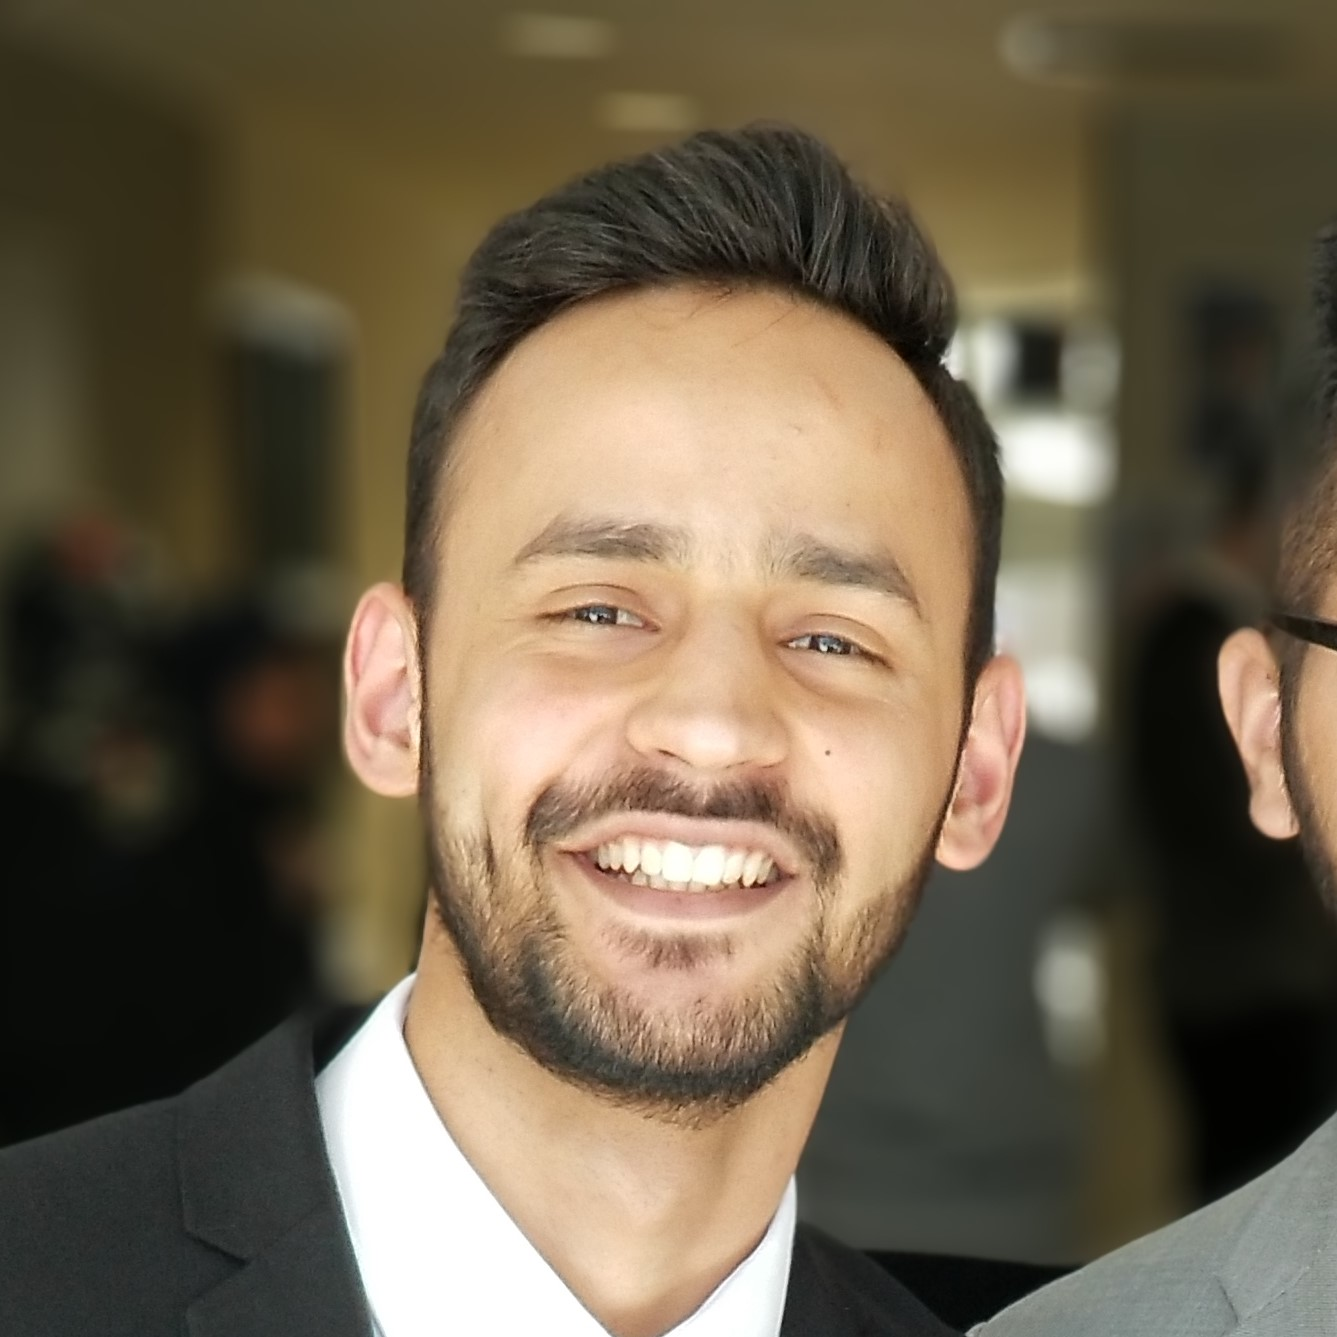
\includegraphics[width=0.17\linewidth]{meh.jpg}};
% \end{tikzpicture}

% \begin{tikzpicture}[remember picture,overlay]
% \clip ($(current page text area.north east)!0.05!(current page text area.south east)!0.07!(current page text area.north west)$)
%   circle (1.5cm) node {
\includegraphics[width=0.16\linewidth]{meh1.jpg}};
% \end{tikzpicture}

%----------------------------------------------------------------------------------
%	LEFT COLUMN
%----------------------------------------------------------------------------------

\begin{minipage}[t]{0.29\textwidth}
\vspace{-5mm}

\section{Skills}
\sectionspace
% \textbullet{} Problem \vspace{1mm} Solver \\
% \\ Team Player
% \textbullet{} Strong Work Ethic  \\ \vspace{1mm} Time management
% \textbullet{} Self-discipline  \\ \vspace{1mm}  
% \textbullet{Critical Thinking} \vspace{1mm} \\
% \textbullet{} Organizational  \vspace{1mm} 

%\sectionsep
% mechanics, design, essential, software, pneumatics 
% \subsection{Design}  \vspace{1mm}
% \subsection{Languages}

% \textbullet  Design and Development of Mechanics \\ \vspace{1mm}
\textbullet   Agile Development \\ \vspace{1mm}
\textbullet  Rest APIs  \\ \vspace{1mm}
\textbullet Design Principles \\ \vspace{1mm}
\textbullet software design patterns \\ \vspace{1mm}
\textbullet User Experience (UX) \\ \vspace{1mm}

\textbullet   Relational Databases \\ \vspace{1mm}
\textbullet   Software Development Life Cycle \\ \vspace{1mm}
\textbullet  Technical Documentation \\ \vspace{1mm}
\textbullet  Real time system design \\\vspace{1mm}
\textbullet  FPGA/Arduino/micro-controllers \\ \vspace{1mm}
% \textbullet  SolidWorks \& AutoCAD \\ \vspace{1mm}
% \textbullet  CAD drawing \\\vspace{1mm}
% \textbullet 2D \& 3D modeling \\\vspace{1mm}

% \textbullet  Design procedures; theories of failure \& material selection \\ \vspace{1mm}
\textbullet  PLC \& embedded system programming \\ \vspace{1mm}

% \textbullet  Analytical \& creative process-thinking \\ \vspace{1mm}
%\textbullet Self-starter \\
% \textbullet  PCB schematic design \\ \vspace{1mm}
% \textbullet  Microsoft Office Suite \\ \vspace{2mm} 

\sectionspace
\subsection{Programming}
\sectionspace
C \thinspace \textbullet{} Node.js \textbullet{} MySQL \textbullet{} Angular.js \\ Python  \thinspace \textbullet{}Java \textbullet{}   C++ \textbullet{}PHP 
\sectionspace
% \subsection{Engineering Analysis Tools}
%  \sectionspace 
% SolidWorks \textbullet{}AutoCAD  \textbullet{}MATLAB \\ LabVIEW \textbullet{} Microsoft Office Suite 
% \sectionspace


\section{Education} 
\sectionspace
\subsection{Ryerson University}
\descript{Bachelor of Mechanical Engineering}
\location{Sept 2014 - Apr 2018}

\section{Coursework}
\sectionspace
\subsection{Undergraduate}
\sectionspace

Intelligent Systems \\ \vspace{1mm}
Microprocessor Systems \\ \vspace{1mm}
% Electric Machines and Actuators\\ \vspace{1mm}
Robotics \\ \vspace{1mm}
Sensors and instrumentation\\ \vspace{1mm}
Digital Systems\\ \vspace{1mm}
% Engineering Design \\ \vspace{1mm}
Project Management\\ \vspace{1mm}
Real-time Operating Systems \\ \vspace{1mm}
% Machine Design\\ \vspace{1mm}
% Manufacturing System Control\\ \vspace{1mm}
% Manufacturing Fundamentals\\ \vspace{1mm}
% Thermodynamics\\ \vspace{1mm}
% Stress Analysis\\ \vspace{1mm}


% \sectionspace
% \subsection {certifications}
% \sectionspace
% Certified SolidWorks Professional \textbf{(CSWP)} \\\vspace{1 mm} Status: Segment 2\&3 passed \\ \hspace{30.5pt} Segment 1 remaining \\\vspace{1 mm} Completion Date: December 2019

%  \vspace{1 mm} Registered with PEO

\sectionspace
\subsection {Online Coursework}
\sectionspace
Mastering Coding Interview (Andrei Neagoie | status: 60\%) 
\\ \vspace{2 mm}
Advanced Javascript Concepts (Udemy| status: In Progress) 
% \\ \vspace{2 mm}
% Introduction to Algorithms (MIT| status: In Progress| Level: Masters) 

\end{minipage} 
\hfill
\begin{minipage}[t]{0.66\textwidth} 

%%%%%%%%%%%%%%%%%%%%%%%%%%%%%%%%%%%%%%
%     EXPERIENCE
%%%%%%%%%%%%%%%%%%%%%%%%%%%%%%%%%%%%%%
\vspace{-5mm}
\section{Relevant Experience}
\sectionspace
\runsubsection{Software Development Lead}
\descript{| PFERA}
\location{June 2018 – Present | Kitchener, ON}
\vspace{\topsep}
\sectionspace
\begin{tightitemize}

\item  Fleshed out a minimal legacy code-base with major enhancements and \textbf{spearheaded} deployment to production resulting in the company’s \textbf{first ever revenue generation} 
\vspace{1mm}
\item \textbf{Responsible for the entire life cycle} of the project from architecture design, development, testing, deployment of web and mobile implemented in \textbf{Vue.JS} (frontend), \textbf{PHP/Laravel} (backend), and \textbf{Ionic} (mobile) with a \textbf{MySQL} database
\vspace{1mm}
\item Designing and developing \textbf{15+ new features} including user side invoicing, custom forms with user templates, auto-scheduler, complete UI update on web and mobile and setting up \textbf{linux} staging server for additional testing purposes
\vspace{1mm}
\item Implementing core infrastructure to incorporate old user records into Rscript learning models to provide helpful insights and accurate time of foaling and creating horse states to link various types of breeding records for multiple learning models to work collaboratively 

\end{tightitemize}

\sectionspace

\runsubsection{Mechatronics Designer}
\descript{| freelance/contract}
\location{Sept 2016– May 2018}
\vspace{\topsep}
\begin{tightitemize}
\item Design and develop wide range of mechanical components and automation systems on contract basis 
\vspace{1mm}
\item Involved in product development for numerous automation systems from developing designs to prototyping and testing, which generated \textbf{revenue of more than \$10k}
\vspace{1mm}
% \item Consulted with clients to determine technical information and project specifications
% \vspace{1mm}
% \item Designed \textbf{CAD models} and drawings for manufacturing
\end{tightitemize}

% \runsubsection{Ryerson Formula SAE}
% \descript{| Power-train Team}
% \location{Oct 2015 – Dec 2017}
% %\vspace{\topsep}
% %\sectionsep
% \begin{tightemize}
% \item Worked with a group of engineering students to design, build, and assemble power-train components such as exhaust systems and intake manifolds\\
% \vspace{1mm}
% \item Utilized simulation softwares SolidWorks and AutoCAD to perform stress and thermodynamic analysis
% \end{tightemize}

%%%%%%%%%%%%%%%%%%%%%%%%%%%%%%%%%%%%%%
%     Projects
%%%%%%%%%%%%%%%%%%%%%%%%%%%%%%%%%%%%%%

\section{PROJECTS}
\sectionspace

% \runsubsection{4-Bar Claw Grabber Mechanism}
% \descript{| Design Project}
% \location{Jan 2016 – Apr 2016}
% %\vspace{\topsep}
% \begin{tightemize}
 
% \item Led a group of 4 members to design a 4-bar mechanism crane to grab and move round objects to designated location
% %\vspace{1mm}
% %\item Created a robust design taking into consideration many factors and constraints such as type of turbine, efficiency, and power generated
% \vspace{1mm}
% %\item Determined best design by doing calculations for different designs on Excel
% %\vspace{1mm}
% \item Conducted thorough R\&D on basics of mechanical arms, gears, and pulleys
% \vspace{1mm}
% \item Simulated on SolidWorks and later imported to AutoCAD for laser cutting
% \end{tightemize}
% \sectionsep 
% \sectionspace

% \runsubsection{Ball Crusher}
% \descript{| Design Project}
% \location{Sept 2017 – Dec 2017}
% % \vspace{\topsep}
% \sectionspace
% \begin{tightitemize}
 
% \item Designed a linear electric actuator with variable force output to grip or crush objects
% \vspace{1mm}
% \item Configured a \textbf{DAQ} to control the linear speed and motion of actuator based on desired force output
% \vspace{1mm}
% \item Designed electrical circuit for motor and power unit of the actuator 
% % \vspace{1mm}
% \item Designed \textbf{CAD models} of actuator parts for 3D printing
% % \vspace{1mm}
% % \item Simulated on SolidWorks and later imported to AutoCAD for laser cutting
% \end{tightitemize}
% \sectionspace





% \runsubsection{Gearbox}
% \descript{| Design Project}
% \location{Jan 2018 – April 2018}
% % \vspace{\topsep}
% % \sectionspace
% \begin{tightitemize}
% % \sectionpace

% \item Developed an efficient gearbox to transfer torque from a 10HP motor to a SOLO air propeller and met required constraints
% \vspace{1mm}
% \item Designed it to be \textbf{operable for $10^7$ life cycles}, withstanding moderate shock, no resonances, as well as all the parts complimenting one another
% \vspace{1mm}
% \item Used an iterative calculations approach for gears, shafts, bearings, and couplings to produce an optimal design and then created it on \textbf{SolidWorks}
% \end{tightitemize}
% \sectionspace


% \runsubsection{POWER PLANT DESIGN}
% \descript{ UNDERGRAD RESEARCH}
% \location{Sept 2016 – Dec 2016}
% % \vspace{\topsep}
% \begin{tightitemize}
% \item Led a team of 4 students to critically analyze and design power plant for use in British Columbia, CA 
% \vspace{1mm}
% \item Created a robust design taking into consideration many factors and constraints such as type of turbine, efficiency, and power generated 
% \vspace{1mm}
% \item Determined best design by doing calculations for different designs on Excel 
% \vspace{1mm}
% \item Increased efficiency in design from \textbf{31.92\% to 45.21\% }and wrote a detailed report on it 
% \end{tightitemize}

\runsubsection{Smart Fire Alarm}
\descript{| Side Project}
\location{April 2018 - May 2018}
\vspace{\topsep}
\begin{tightitemize}
%\sectionsep 

\item Designed a WIFI enabled smoke/CO alarm which relays the occupancy of each room to emergency personnel in event of a fire to \textbf{reduce rescue times} by eliminating the need to search rooms using \textbf{IOT}
\vspace{1mm}
\item Designed occupancy detection subsystem capable of working in robust environments with \textbf{85\% reliability} coded in \textbf{C on Arduino and ESP8266}
\vspace{1mm}
% \item Designed PCB schematics using OrCAD for manufacturing 
% \vspace{1mm}
\item Developed and conducted \textbf{custom hardware \& software tests} to validate system for high reliability
\end{tightitemize}
\sectionspace



% \runsubsection{PLC Manufacturing}
% \descript{| Design Project}
% \location{Jan 2018 – April 2018}
% \vspace{\topsep}
% \begin{tightitemize}
% %\sectionsep 

% \item Designed, with a team, a fully \textbf{automated production process} to manufacture photo certificates to increase production 
% \vspace{1mm}
% \item Developed \textbf{PLC ladder logic} to program switches, actuators, laser and machine vision sensors to control a sequential manufacturing
% operation using Allen Bradley
% \vspace{1mm}
% % \item Developed the ladder logic in \textbf{Omron} syntax and flowchart as well to track all the manufacturing processes in \textbf{Microsoft Visio}
% \end{tightitemize}
% \sectionspace

\runsubsection{Autonomous Guided Vehicle}
\descript{| Side Project}
\location{Jan 2017 – Dec 2017}
\vspace{\topsep}
\begin{tightitemize}
% \item Designed a \textbf{fully autonomous robot} capable of transporting material with an aim to increase worker safety and efficiency 
% \vspace{1mm}
\item Developed algorithms in \textbf{C} to detect and handle obstacles such as color, luminous flux, multiple lines, sound frequencies, objects, and walls utilizing encoders and various sensors to solve complex mazes and navigate through obstacles
\vspace{1mm}
\item Designed a 3-DOF robotic arm with a cylindrical work envelope using servo motors to grab material securely.
% \vspace{1mm}
% \item Drafted a design report, using engineering report writing standards 
%\item Programmed an EVshield to control a crane built with NXT to wind up or down a weight with a button and calculate its average velocity
\end{tightitemize}

% \runsubsection{UAV Parcel delivery design}
% \descript{| Research}
% \location{Jan 2017 – Dec 2017}
% \vspace{\topsep}
% \begin{tightitemize}
% \item Designed a vibration absorber to meet certain criteria and reduce vibration from UAV drone to parcel
% \vspace{1mm}
% \item Created MATLAB scripts to model natural frequencies, and steady state vibration amplitude of system components at any given time
% \vspace{1mm}
% \item Developed MATLAB algorithms to process various constraints to produce design dimensions that satisfy said constraints and simulated them on \textbf{SolidWorks}
% \vspace{1mm}
% \item Built robot arm with NXT to grip and moving different objects to different locations, through having the program algorithms account for physical properties of object, such as weight, shape, size, and color
% \vspace{1mm}
% \item Programmed an EVshield to control a crane built with NXT to wind up or down a weight with a button and calculate its average velocity
% \end{tightitemize}

\runsubsection{Digital PID Controller}
\descript{| Research Project}
\location{Jan 2018 – Apr 2018}
\vspace{\topsep}
\begin{tightitemize}
 
\item Designed and implemented a real-time digital anti-windup and basic PID controller to control position of DC motor using \textbf{concurrent programming in C}

% \vspace{1mm}

% \item Programmed and debugged on \textbf{RTOS} using \textbf{Pthreads} and various kernel objects like semaphores and mutexes to increase reliability
\end{tightitemize}
\sectionspace


\end{minipage} 
\end{document}  \documentclass[]{article}